\documentclass{article}
\usepackage[utf8]{inputenc}

\usepackage{amsmath}
\usepackage{amssymb}
\usepackage{amsthm}

\usepackage{subfig}
\usepackage{graphicx}
\usepackage{float}

\usepackage{mathtools}
\DeclarePairedDelimiter{\ceil}{\lceil}{\rceil}
\DeclarePairedDelimiter{\floor}{\lfloor}{\rfloor}

\title{DQ-N Spec}
\author{Keyi Zhang}
\date{April 2017}

\begin{document}


There are three major components in a DQ-N frame, namely, TR slots, data frames, and feedback frames, as shown in Figure~\ref{fig:improved-frame}. Currently two transmission rates are supported. Without explicitly mentioning transmission rate, all packets are transmitted using the slower radio modem configuration. Each node is allowed to request up to 2 data slots.

\begin{figure}[htb]
 \centering 
 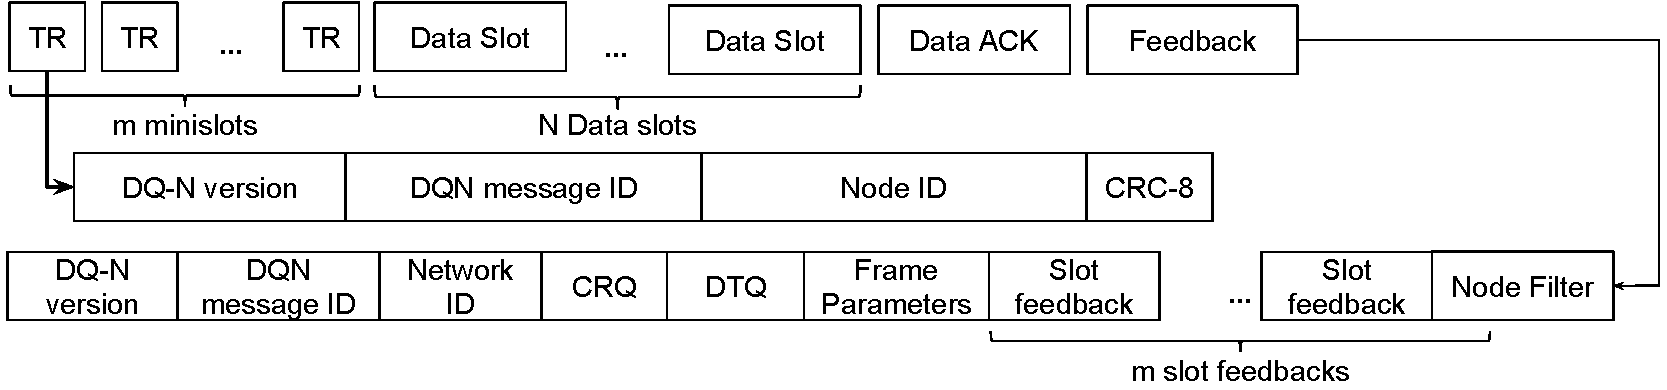
\includegraphics[width=1\linewidth]{improved-frame.pdf}
 \caption{DQ-N frame structure.}
\label{fig:improved-frame}
\end{figure}

One thing to notice is that the entire network can be reconfigured at run time, which can be done at the synchronization state, as shown in Section \ref{app:sec:sync}. This is done by encoding network information into the feedback packet. In addition, since this version is implemented on LoRa radio, there are some extra details we need to take care of. LoRa radio by default will include a header and CRC-8 at the end. To save space and enable collision detection, the protocol requires no header and no CRC mode in TR transmission. However, for normal transmission, we can use the built-in CRC to drop corrupted packets automatically.

\section{Protocol Overview}
This section describes the behaviors of the node and server, including registration and how to send and receive data from the network.

\subsection{Node Synchronization}
\label{app:sec:sync}
Before transmitting any data to the server, the node has to synchronize its clock to the server's. To do so, it will continue listening to the channel until it receives a valid feedback packet. It then calculate all the DQ-N parameters encoded in the feedback packet and length for each sub-frames. Using these values the device can compute the time when the frame starts and thus finish the synchronization.

To take clock drifting into account, the node needs to remember the last time when it synchronized with the base station. If it has been too long, i.e. the current timestamp minus last synchronized time exceeds predefined threshold, the node has to synchronize again before sending any data.

To change the network configuration at run time, the base station needs to make sure DTQ has to be empty so that no data will be lost. To do so, the base station will set CRQ length value in the feedback to be maximum value. Therefore every device has to enter DTQ and sleep. Given the size of CRQ values, it is easy to put all devices out of synchronization. Hence once these nodes try to sending data to the newly reconfigured network, they have to synchronize again and obtain the new network configuration.

\subsection{Node Joining Process}
To join, the node has to send a special TR request, asking for two data slots. Once TR is successfully sent, the device will enter DTQ. At the first data slot, the device will send a join packet containing its hardware address. At the second data slot, the base station will send a join response with a node ID assigned to that node. Once the node obtains its node ID, the joining process is finished. The TR is sent without a header and CRC using slow transmission rate.

\subsection{Node Sending and Receiving Data}
Sending and receiving data is very similar to the joining process except the Message ID attributes (see Section~\ref{app:sec:frame}) are different. Currently there is no downstream flag in the feedback and the node has to actively request downstream packets by sending corresponding TRs.

\subsection{Protocol Sequence Example}
An overview of the joining and sending process is shown in Figure~\ref{fig:dqn-seq}. Figure~\ref{fig:dqn-join} shows that the node listens to feedback and decodes the network information as well as synchronizing the clock. Then it sends a TR-JOIN (a special TR) to the base station. TR-JOIN is successfully received by the base station and the device enters DTQ immediately. Upon sending packets, the node first sends its entire hardware address, then receives the assigned node ID. Figure~\ref{fig:dqn-send} shows how a device sends data to the base station. First it sends a TR. Unfortunately there is a contention and the device has to enter CRQ. After another TR request the device successfully enters DTQ. When it is the device's turn to transmit, it sends data to the base station.

\begin{figure}[htb]
     \centering
     \subfloat[][DQ-N joining procedure.]{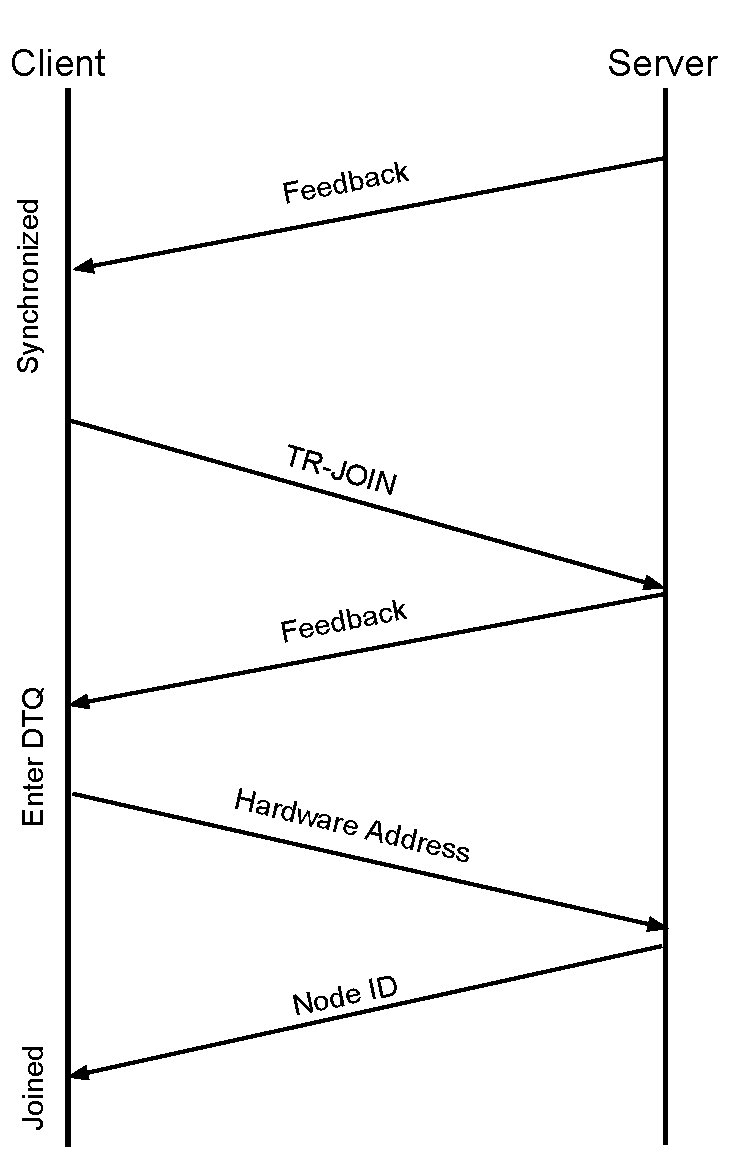
\includegraphics[width=0.4\textwidth]{DQN-JOIN.pdf}\label{fig:dqn-join}}
     \subfloat[][DQ-N send procedure. Notice that the first TR has a contention and as a result, another TR needs to be sent.]{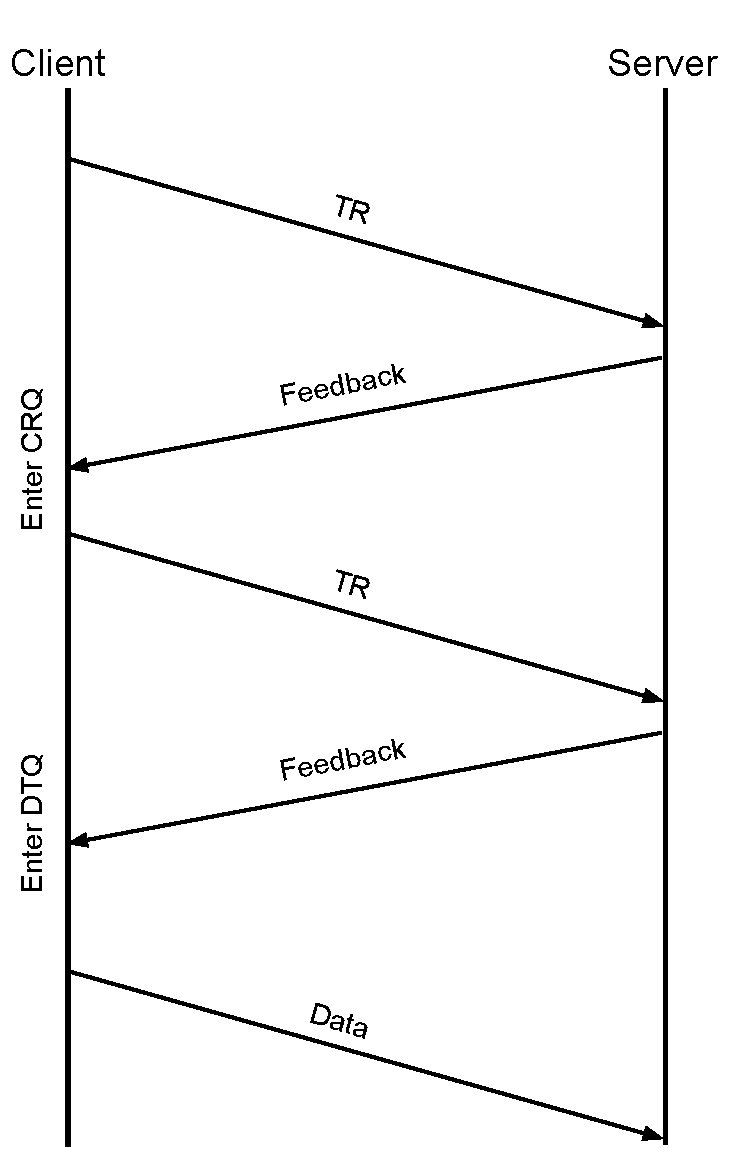
\includegraphics[width=0.4\textwidth]{DQN-SEND.pdf}\label{fig:dqn-send}}
     \caption{DQ-N protocol sequence diagram.}
     \label{fig:dqn-seq}
\end{figure}

\section{Frame Details and Equation}
\label{app:sec:frame}
To calculate the size of a Node Filter, which is essentially a bloom filter, the following equation is used to calculate the size given a specific error rate and entry size.
\begin{align}
\label{eqn:node_filter}
m = n\log_2e\cdot \log_2(1/\epsilon),
\end{align}
where $\epsilon$ is the false positive (error) rate and $n$ is the number of entries. The error rate will be encoded into the feedback back and $n$ is simply the number of TRs per frame.

For all protocol messages, the version has to be 0x27 and the message id has to be one of the following listed in Table \ref{table:messageid}.

The structures for TR, feedback, JOIN-REQ, and JOIN-RESP are shown in Table \ref{app:structure:tr} \ref{app:structure:feedback}, \ref{app:structure:join-req}, and \ref{app:structure:join-resp}, respectively. Notice that TR-JOIN shares the same structure as TR, yet the Node ID will be set to 0 and the message ID will be different. For a TR, upper 4 bits of message ID are fixed and the lower 4 bits carry the TR request information is shown in Table \ref{app:table:low-bits}.




\begin{table}[H]
\centering
\caption{MessageID values table for DQ-N version 0.27}
\label{table:messageid}
\begin{tabular}{|c|c|}
\hline
Type      & Value/Mask \\ \hline \hline
TR        & 0x8X       \\ \hline
Feedback  & 0x01       \\ \hline
TR-JOIN   & 0x92       \\ \hline
JOIN-REQ  & 0xA0       \\ \hline
JOIN-RESP & 0xA1       \\ \hline
\end{tabular}
\end{table}

\begin{table}[H]
\centering
\caption{TR structure for DQ-N version 0.27}
\label{app:structure:tr}
\begin{tabular}{|c|c|}
\hline
Attribute   & Size  \\ \hline \hline
DQN version   & 1 Byte  \\ \hline
DQN MessageID & 1 Byte  \\ \hline
NodeID        & 2 Bytes \\ \hline
CRC           & 1 Byte  \\ \hline
\end{tabular}
\end{table}


\begin{table}[H]
\centering
\caption{Feedback structure for DQ-N version 0.27}
\label{app:structure:feedback}
\begin{tabular}{|c|c|}
\hline
Attribute   & Size  \\ \hline \hline
DQ-N Version      & 1 Byte                 \\ \hline
DQ-N MessageID    & 1 Byte                 \\ \hline
DQ-N NetworkID    & 4 Bytes                \\ \hline
Unix Timestamp   & 4 Bytes                \\ \hline
CRQ Length       & 2 Bytes                \\ \hline
DTQ Length       & 2 Bytes                \\ \hline
Frame Parameters & 2 Bytes                \\ \hline
Slots            & Determined by Equation \\ \hline
Node Filter      & Determined by Equation \ref{eqn:node_filter} \\ \hline
\end{tabular}
\end{table}

\begin{table}[H]
\centering
\caption{TR-JOIN structure for DQ-N version 0.27}
\label{app:structure:tr-join}
\begin{tabular}{|c|c|}
\hline
Attribute   & Size  \\ \hline \hline
DQN version   & 1 Byte  \\ \hline
DQN MessageID & 1 Byte  \\ \hline
Hardware Address    & 6 Bytes \\ \hline
\end{tabular}
\end{table}

\begin{table}[H]
\centering
\caption{JOIN-REQ structure for DQ-N version 0.27}
\label{app:structure:join-req}
\begin{tabular}{|c|c|}
\hline
DQN version   & 1 Byte  \\ \hline
DQN MessageID & 1 Byte  \\ \hline
Hardware Address    & 6 Bytes \\ \hline
\end{tabular}
\end{table}

\begin{table}[H]
\centering
\caption{JOIN-RESP structure for DQ-N version 0.27}
\label{app:structure:join-resp}
\begin{tabular}{|c|c|}
\hline
Attribute   & Size  \\ \hline \hline
DQN version   & 1 Byte  \\ \hline
DQN MessageID & 1 Byte  \\ \hline
Hardware Address    & 6 Bytes \\ \hline
NodeID        & 2 Bytes \\ \hline
\end{tabular}
\end{table}


\begin{table}[H]
\centering
\caption{Message ID values for TR structure}
\label{app:table:low-bits}
\begin{tabular}{|c|c|c|}
\hline
Name      & Bits & Description \\ \hline \hline
Num slots & 0-1  & 0, 1, 2                                                          \\ \hline
Up/down   & 2    & 0 = upstream to base, 1 = downstream to node                     \\ \hline
Rate      & 3    & 0 is low trans rate and 1 is high rate \\ \hline
\end{tabular}
\end{table}

The frame parameter in Feedback is defined in Table \ref{app:table:frame-parameter}.

\begin{table}[H]
\centering
\caption{Encoding details of frame parameters in feedback structure}
\label{app:table:frame-parameter}
\begin{tabular}{|c|c|c|c|}
\hline
Name & Bits  & Description  \\ \hline \hline
FPP  & 0-1   & False Positive Probability (0=0.1\%, 1=1\%, 2=2\%, 3=5\%) \\ \hline
TRF  & 2-7   & TRs per Frame $= 16+4\times TRF $                                              \\ \hline
DTR  & 8-11  & Data Slots per TR, number of data slots $= \floor{\frac{DTR}{15} (16+4\times TRF)}$                  \\ \hline
MPL  & 12-15 & Max payload in bytes $=6 \times(MPL+1)$                     \\         \hline     
\end{tabular}
\end{table}

\end{document}
